\documentclass{article}
\usepackage[utf8]{inputenc}
\usepackage{mathtools}
\usepackage{graphicx}
\usepackage{hyperref}

\setlength{\parindent}{0pt}

\title{AerE 161 \\ Project \#1: Standard Atmosphere Table}
\author{Hammad Imam \\ Undergraduate, Aerospace Engineering \\ Iowa State University}
\date{February 23rd, 2018}

\begin{document}

\begin{titlepage}
\maketitle
\end{titlepage}

\clearpage
\tableofcontents

\section{Problem Statement}
The purpose of this project was to generate a Standard Atmosphere Table, with values for the standard atmosphere from the troposphere to the stratosphere. The table outputs the geopotential altitude from 0 to 47km in steps of 1km, and uses those values to find the geometric altitude, and standard values for temperature, density, and pressure. Additionally, three graphs were generated, plotting temperature, density, and pressure all against the geopotential altitude. 

\section{Theory}
\subsection{Introduction}
In this section, the methods of calculations for each calculated value will be explained. There are three parts of the atmosphere that all behave differently, so each subsection will explain what was done differently for each value. Any constants used in calculations will be expressed in the subsection that uses those constants. Every subsection will contain a short overview of the value, and then calculations for the value derived from the hydrostatic equation and equation of state. The calculations will all be either in terms of the geopotential altitude $h$, or of a previously calculated value. All work and explanations will be shown, and final results for a formula will have a number displayed next to them.

\subsection{Geometric Altitude, \texorpdfstring{$h_g$}{}, m}
Geometric altitude $h_g$ is the "true" distance off the surface of the Earth, as opposed to geopotential altitude $h$ which is a "fictitious" altitude that represents the height with an assumption of constant gravitational acceleration $g_0$, as opposed to one that varies with the distance from the surface.\\
Geometric altitude $h_g$ is related to geopotential altitude $h$ by the formula 
\begin{align}
    h_g &= \frac{h * r_E}{r_E - h}
\end{align}
where $r_E$ represents the radius of Earth, $6371.0008 km$. In the Standard Atmosphere Table, the geometric altitude is calculated directly from the stepped geopotential altitude.

\subsection{Temperature, \texorpdfstring{$T$}{} , K}
Temperature $T$ is displayed in the table in units Kelvin. The temperature first decreases in the troposphere, remains constant in the isothermal layer, and then rises again in the stratosphere. Layers where the temperature changes are referred to as "gradient layers." \\
The equation given from the hydrostatic equation is as follows

\begin{align*}
    T &= T_1 + a(h - h_1)
\end{align*}
where $T_1$ is the temperature 1 lower than the value being calculated, $a$ is the lapse rate $\frac{dT}{dh}$, $h$ is the current height, and $h_1$ is the height 1 lower than the value being calculated. \\ 
Since the equation depends on lower values of the temperature, an initial temperature is required to calculate higher values. $T_0$, the temperature at sea level, is given as 

\begin{align*}
    T_{0} &= 288.16 K \\
\end{align*}
The values for $a$, the lapse rate of the temperature, depend on the layer of atmosphere. The values are given below

\begin{align*}
    a &= \begin{cases}
    -6.5\times10^{-3}\  K/m   & troposphere,\ h = [0,11] \\
    0 \ K/m                  & isothermal,\ h = [12,24] \\
    3\times10^{-3}\ K/m     & stratosphere,\ h = [25,47] \\
    \end{cases}
\end{align*}
The geopotential altitude in the table is calculated in steps of 1km, so the value for $(h-h_1)$ will remain a constant 1km.\\
Inserting these values into the original equation for temperature gives us the combined equation

\begin{align}
    T_h &= \begin{cases}
    T_{h-1}\ K - (6.5\times10^{-3}\  K/m)(1km)    & troposphere,\ h = [0,11] \\
    T_{h-1} \ K                                          & isothermal,\ h = [12,24] \\
    T_{h-1}\ K + (3\times10^{-3}\ K/m)(1km)       & stratosphere,\ h = [25,47] \\
    \end{cases}
\end{align}

\subsection{Density, \texorpdfstring{$\rho$}{}, kg/m\texorpdfstring{$^3$}{} }
Density $\rho$ is displayed in the table in units kg/m$^3$. The rate of change is reliant on the ratio between the temperature at the current height, so a different formula must be used for the isothermal layer than from the gradient layers. The original equations are 

\begin{align*}
    \frac{\rho}{\rho_1} &= {\left(\frac{T}{T_1}\right)}^{-\frac{g}{aR}-1} \\
    \frac{\rho}{\rho_1} &= e^{\left(- \frac{g}{RT}\right)\left(h-h_1\right)}
\end{align*}

where gravitational acceleration $g = 9.81m/s^2$, lapse rate $a= -6.5\times10^{-3} K/m$ in the troposphere and $3\times10^{-3}K/m$ in the stratosphere, and $R = 287 \frac{J}{kg\ K}$. The first equation is used in the gradient layers, while the second equation is used in the isothermal layers. With some rearranging, the equations become

\begin{align*}
    \rho_h &= \rho_{h-1}{\left(\frac{T_h}{T_{h-1}}\right)}^{-\frac{g}{aR}-1} \\
    \rho_h &= \rho_{h-1}\left(e^{\left(- \frac{g}{RT}\right)\left(h-h_1\right)}\right)
\end{align*}

Since each value will be calculated, temperature values will be independently calculated in each row and used in the formula for density. Gravitational acceleration $g$, lapse rate $a$, and specific gas constant $R$ are all known values. The geopotential altitude in the table is calculated in steps of 1km, so the value for $(h-h_1)$ will remain a constant 1km. Subbing in all known values gives the equation 

\begin{align}
    \rho_h &= \begin{cases}
    \rho_{h-1}{\left(\frac{T_h}{T_{h-1}}\right)}^{\frac{9.81 m/s^2}{6.5\times10^{-3}K/m\ 287 \frac{J}{kg\ K}}-1}    & troposphere,\ h = [0,11] \\
    \rho_{h-1}\left(e^{\left(- \frac{9.81 m/s^2}{T_h * 287 \frac{J}{kg\ K} }\right)\left(1 km\right)}\right)                                          & isothermal,\ h = [12,24] \\
    \rho_{h-1}{\left(\frac{T_h}{T_{h-1}}\right)}^{-\frac{9.81 m/s^2}{3\times10^{-3}K/m\ 287 \frac{J}{kg\ K}}-1}       & stratosphere,\ h = [25,47] \\
    \end{cases}
\end{align}

\subsection{Pressure, \texorpdfstring{$p$}{}, N/m}
Pressure $p$ is displayed in the table in units N/m. Similar to density, he rate of change is reliant on the ratio between the temperature at the current height, so a different formula must be used for the isothermal layer than from the gradient layers. The original equations are 

\begin{align*}
    \frac{p}{p_1} &= {\left(\frac{T}{T_1}\right)}^{-\frac{g}{aR}} \\
    \frac{p}{p_1} &= e^{\left(- \frac{g}{RT}\right)\left(h-h_1\right)}
\end{align*}

where gravitational acceleration $g = 9.81m/s^2$, lapse rate $a= -6.5\times10^{-3} K/m$ in the troposphere and $3\times10^{-3}K/m$ in the stratosphere, and $R = 287 \frac{J}{kg\ K}$. The first equation is used in the gradient layers, while the second equation is used in the isothermal layers. Rearranged, the equations become 

\begin{align*}
    p &= p_{h-1}{\left(\frac{T_h}{T_{h-1}}\right)}^{-\frac{g}{aR}} \\
    p_h &= p_{h-1}\left(e^{\left(- \frac{g}{RT}\right)\left(h-h_1\right)}\right)
\end{align*}

Since each value will be calculated, temperature values will be independently calculated in each row and used in the formula for pressure. Gravitational acceleration $g$, lapse rate $a$, and specific gas constant $R$ are all known values as listed above. The geopotential altitude in the table is calculated in steps of 1km, so the value for $(h-h_1)$ will remain a constant 1km. Replacing variables for all known values gives the equation

\begin{align}
    p_h &= \begin{cases}
    p_{h-1}{\left(\frac{T_h}{T_{h-1}}\right)}^{\frac{9.81 m/s^2}{6.5\times10^{-3}K/m\ 287 \frac{J}{kg\ K}}}    & troposphere,\ h = [0,11] \\
    p_{h-1}\left(e^{\left(- \frac{9.81 m/s^2}{T_h * 287 \frac{J}{kg\ K} }\right)\left(1 km\right)}\right)                                          & isothermal,\ h = [12,24] \\
    p_{h-1}{\left(\frac{T_h}{T_{h-1}}\right)}^{-\frac{9.81 m/s^2}{3\times10^{-3}K/m\ 287 \frac{J}{kg\ K}}}       & stratosphere,\ h = [25,47] \\
    \end{cases}
\end{align}

\clearpage
\section{Solution}

\subsection{Overview}

This section will contain the code used to generate the standard atmosphere table, the table itself, and the 3 plots of temperature $T$, density $\rho$, and pressure $p$ all against geopotential altitude $h$. The code section will contain screenshots of the code as it appears in the MATLAB editor. The Standard Atmosphere Table section will contain the table as it appears in the MATLAB output, with line breaks added for readability. The plots section will contain the graphs exactly as they are generated in the MATLAB output.

\subsection{Code}
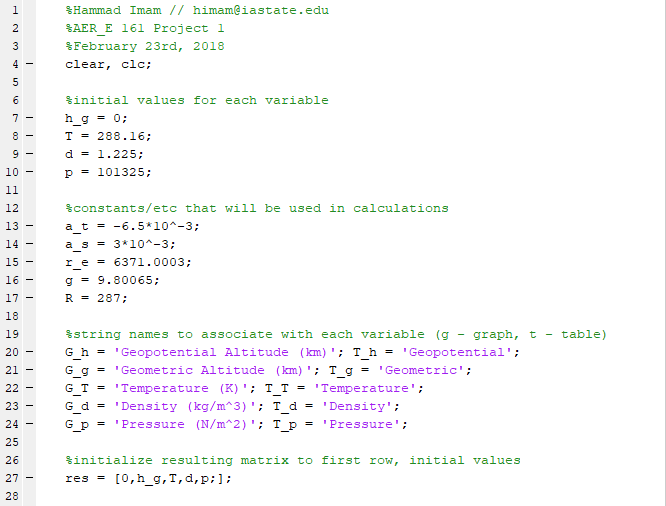
\includegraphics [width=\linewidth]{code1.png}

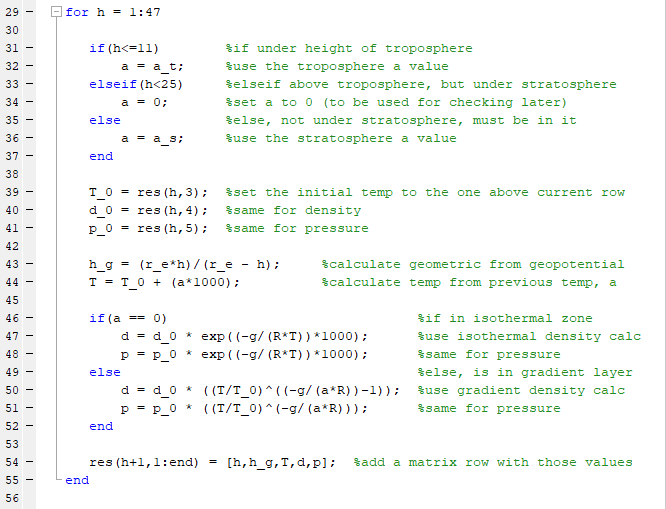
\includegraphics [width=\linewidth]{code2.png}\\
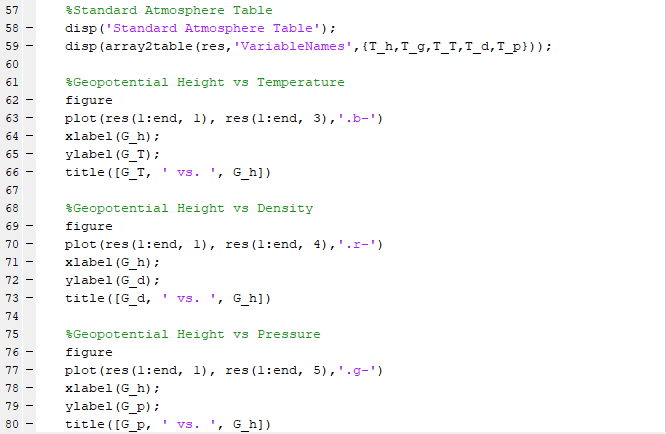
\includegraphics [width=\linewidth]{code3.png}

\newpage
\subsection{Standard Atmopshere Table}
        \begin{verbatim}
    Geopotential    Geometric    Temperature     Density      Pressure 
    ____________    _________    ___________    _________    __________

     0                   0       288.16             1.225    1.0133e+05
     1              1.0002       281.66            1.1117         89880
     2              2.0006       275.16            1.0066         79504
     3              3.0014       268.66           0.90927         70120
     4              4.0025       262.16           0.81932         61654
     
     5              5.0039       255.66           0.73633         54036
     6              6.0057       249.16           0.65993         47198
     7              7.0077       242.66           0.58974         41078
     8              8.0101       236.16           0.52542         35617
     9              9.0127       229.66            0.4666         30760
    
    10              10.016       223.16           0.41296         26453
    11              11.019       216.66           0.36417         22648
    12              12.023       216.66           0.31107         19345
    13              13.027       216.66           0.26571         16524
    14              14.031       216.66           0.22696         14115
    
    15              15.035       216.66           0.19387         12057
    16               16.04       216.66            0.1656         10299
    17              17.045       216.66           0.14145        8796.8
    18              18.051       216.66           0.12082          7514
    19              19.057       216.66            0.1032        6418.3
    
    20              20.063       216.66          0.088155        5482.4
    21              21.069       216.66            0.0753          4683
    22              22.076       216.66           0.06432        4000.1
    23              23.083       216.66          0.054941        3416.8
    24              24.091       216.66          0.046929        2918.6
    
    25              25.098       219.66          0.039581        2495.7
    26              26.107       222.66          0.033461        2138.6
    27              27.115       225.66          0.028351        1836.4
    28              28.124       228.66          0.024074        1580.1
    29              29.133       231.66          0.020485        1362.2
    
    30              30.142       234.66          0.017468        1176.6
    31              31.152       237.66          0.014926        1018.2
    32              32.162       240.66          0.012778        882.72
    33              33.172       243.66          0.010961        766.62
    34              34.182       246.66         0.0094197        666.94
    
    35              35.193       249.66         0.0081101         581.2
    36              36.205       252.66          0.006995        507.31
    37              37.216       255.66         0.0060438        443.53
    38              38.228       258.66         0.0052309        388.37
    39               39.24       261.66         0.0045348         340.6
    
    40              40.253       264.66         0.0039378        299.15
    41              41.266       267.66         0.0034248        263.13
    42              42.279       270.66         0.0029833        231.78
    43              43.292       273.66         0.0026027        204.44
    44              44.306       276.66          0.002274        180.58
    
    45               45.32       279.66         0.0019897        159.72
    46              46.335       282.66         0.0017434        141.45
    47              47.349       285.66         0.0015298        125.4
\end{verbatim}
\subsection{Plots}
\subsubsection{Temperature vs Geopotential Altitude}
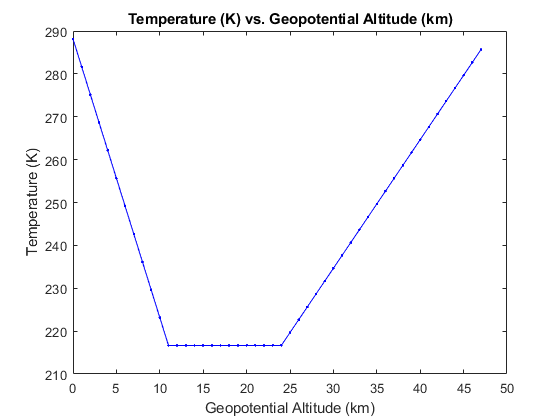
\includegraphics [height=3in]{graph1.png}

\subsubsection{Density vs Geopotential Altitude}
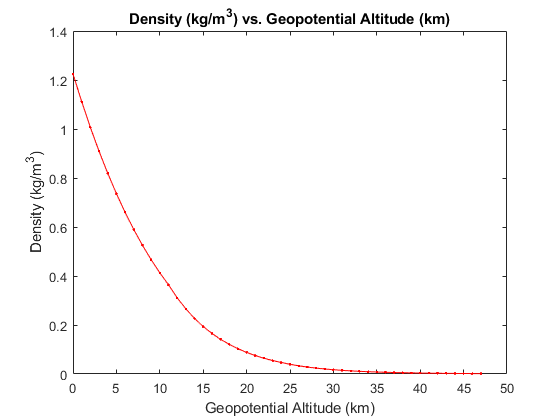
\includegraphics [height=3in]{graph2.png}

\subsubsection{Pressure vs Geopotential Altitude}
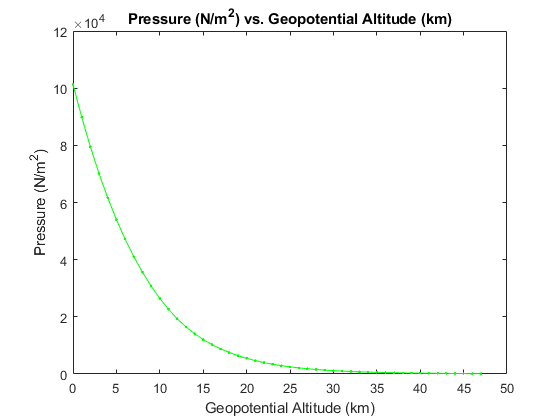
\includegraphics [height=3in]{graph3.png}

\section{Discussion}
\subsection{Analysis}
The geometric height is fairly close to the geopotential height, as throughout the table, the geometric height varies from the geopotential height by a small amount. As visible on the graphs, temperature changes differently from either density or pressure. Temperature starts at a constant value at sea level, then decreases linearly through the troposphere, hits a value of $216.66\ K$ in the isothermal layer, and rises linearly through the stratosphere at a different lapse rate. The density and pressure both decrease fairly smoothly throughout the layers, albeit at different rates to each other, and different rates through the gradient and isothermal layers. The graphs overall show that the air temperature decreases the farther you get from the surface of the earth, but then warms as the atmosphere thins and the air is more directly heated by the sun. The density and pressure of the air both decrease sharply when coming off the Earth, but then decrease at a steadier rate the further off the Earth they get until they'd eventually reach a point where the atmosphere is negligible.

\subsection{Challenges}
This project, as beautiful as it may look, actually took me quite a bit of effort both in coding the MATLAB file, writing this \LaTeX\ document, and uploading it to a GitHub repository. One of the challenges I faced was the formatting on the table of values while using the array2table() function. The spacing for the column headers had a smaller maximum width than the width of the names I had originally planned to use, so I had to create separate strings with shorter names that would fit into the table. I also had some issue with indexing, as my initial draft of the code read the initial row as row 0 when it should have been row 1, which was resolved by writing to the array at the value of the for loop plus one. When writing the \LaTeX\ document, I had a lot of issues with properly formatting the equation and had to look up a good amount of how to type what I was typing. When working with the GitHub repository (available at \url{https://github.com/himam99/AERE161-Project1}), I was mostly reliant on GitHub's cheet sheet, and had some issues pushing to GitHub, so I had to Google that as well. Overall, aside from some minor coding issues, the project wasn't too difficult to complete, if a bit tedious. 
\end{document}
